\documentclass[journal,onecolumn]{IEEEtran}
\usepackage{amsmath,amssymb,booktabs,array,graphicx,url}
\title{Supplementary Material: Cross-Sequence Service Qualification and Delivery Remediability for Frozen IoT Digital Twins}
\author{Shreyas Udaya}
\begin{document}
\maketitle

\section{Source Hierarchy and Protocol}
The primary analysis uses 30 frozen V2 trajectories from ten held-out i2Nav physical sequences and three seeds per sequence. Saved states are on a 10-Hz local ENU clock. Physical sequence is the independent unit; timestamps, seeds, services, delivery cells, source phases, and twin configurations are nested sensitivity variants. Source hashes and settings are recorded in \texttt{results/service\_timing\_budget/protocol\_manifest.json} and \texttt{results/service\_timing\_robustness/protocol\_manifest.json}. No twin was retrained or selected using timing outcomes.

\section{Per-Service Held-Out Comparisons}
At the nominal 30\% pooled acceptance target, the five nested-LOSO methods have the following accepted/false-qualified counts. Cells within a service are not independent experiments.
\begin{table}[h]
\centering\scriptsize
\caption{Accepted; false/accepted by service at the same overall operating-point target. A dash means no accepted cells. Within-service acceptance is generally unmatched.}
\begin{tabular}{lrrrrr}
\toprule
Service & Surface & Identity & AoI & Kinematic & Logistic \\
\midrule
Local 1 s & 90; 1/90 & -- & -- & 28; 0/28 & 68; 12/68 \\
Local 5 s & 54; 4/54 & -- & 40; 0/40 & 28; 0/28 & 56; 16/56 \\
Local 10 s & 82; 5/82 & 200; 82/200 & 142; 29/142 & 39; 6/39 & 75; 12/75 \\
Global & -- & -- & 40; 24/40 & 146; 97/146 & 36; 26/36 \\
\bottomrule
\end{tabular}
\end{table}
Service identity ties all 20 delivery cells of a given service. A matched within-service identity comparison is therefore unavailable. With a predeclared five-percentage-point tolerance for achieved acceptance, only surface-versus-logistic comparisons for local 5 s and 10 s are near-matched; both paired ten-sequence bootstrap intervals cross zero. The exact intervals and all tested acceptance targets are in \texttt{per\_service\_paired\_bootstrap.csv}. Nominal 10\% and 50\% targets are not treated as matched-risk evidence when score discreteness prevents comparable acceptance.
\begin{figure}[h]
\centering
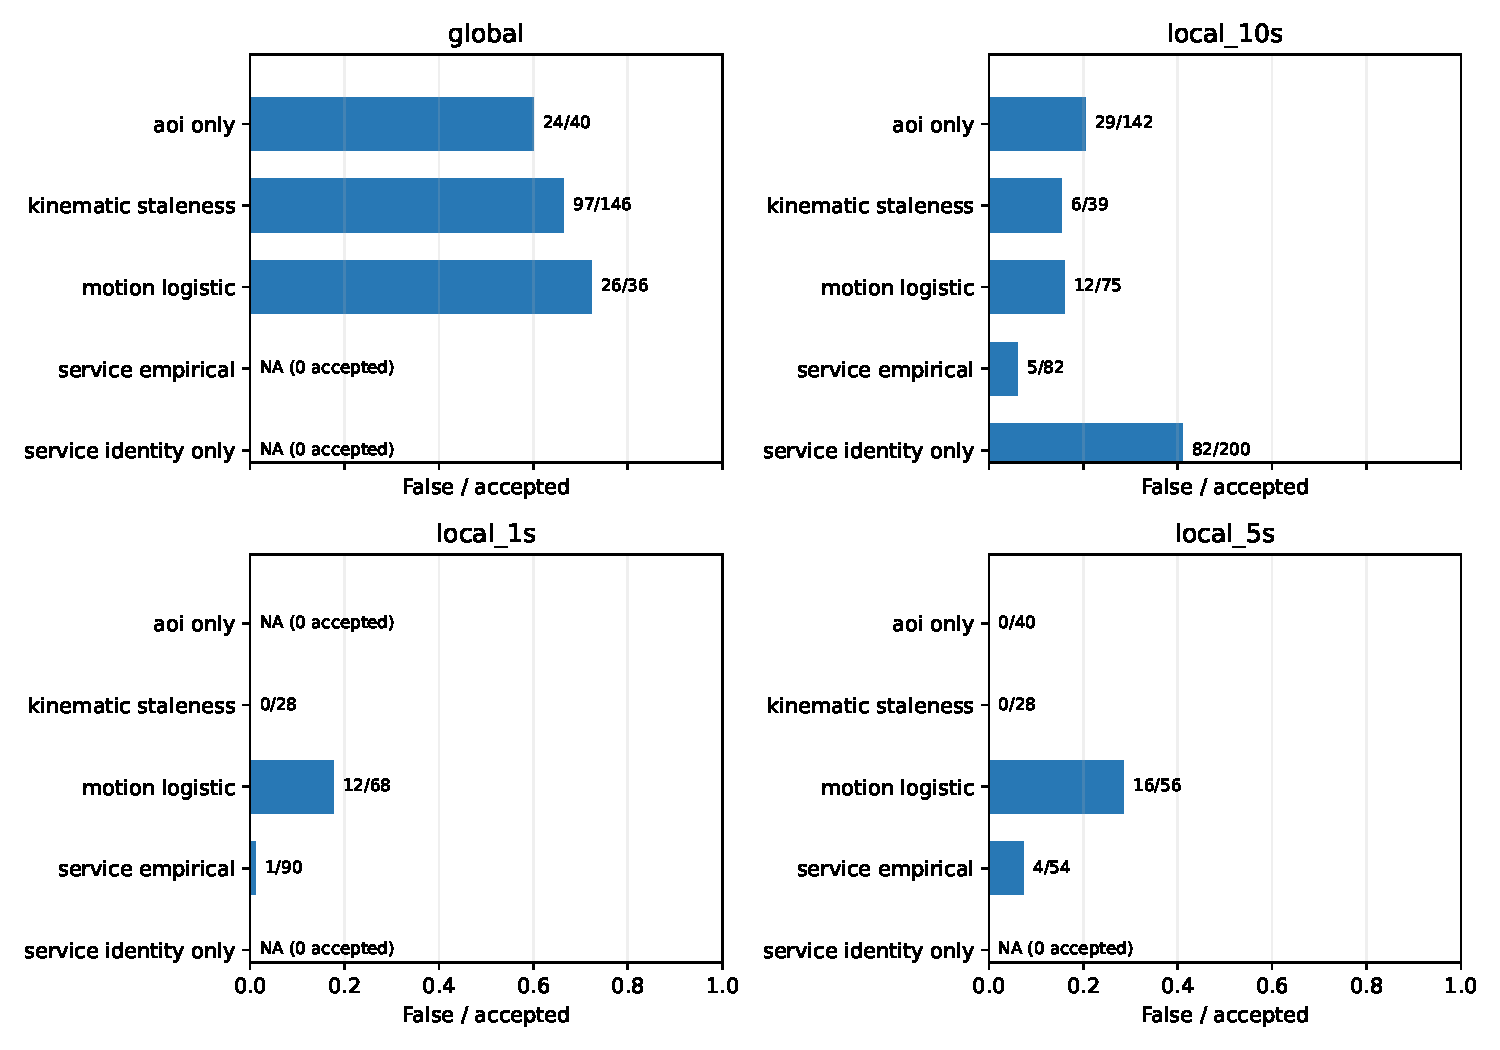
\includegraphics[width=.9\linewidth]{../figures/per_service_qualification.pdf}
\caption{Per-service qualification at the overall 30\% target. Different accepted-cell counts within a service preclude most paired within-service risk claims.}
\end{figure}

\begin{figure}[h]
\centering
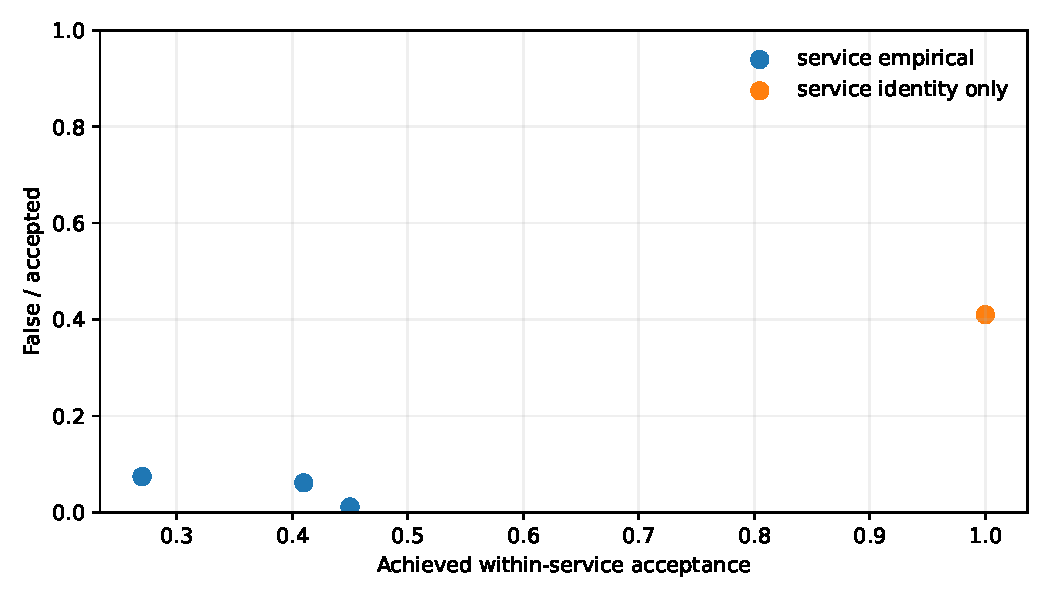
\includegraphics[width=.8\linewidth]{../figures/surface_vs_identity.pdf}
\caption{Pooled cross-sequence surface versus tied service-identity score. Acceptance is approximately, not exactly, matched.}
\end{figure}

\section{Contract-Requirement Sensitivity}
\begin{table}[h]
\centering
\caption{Case partition under predeclared illustrative joint-satisfaction requirements. The 0.80 row is primary; others are sensitivity settings, not safety thresholds.}
\begin{tabular}{rrrr}
\toprule
Requirement & Already qualified & Delivery-remediable & Persistent under ideal \\
\midrule
0.70 & 9 & 26 & 5 \\
0.80 & 3 & 31 & 6 \\
0.90 & 1 & 30 & 9 \\
\bottomrule
\end{tabular}
\end{table}
The distinction persists, but exact case counts depend materially on the illustrative requirement. No neighboring physical-unit discrepancy tolerance grid was frozen for this replay; none was selected after inspection.

\section{Failure Components and Practical Recovery}
The 40 sequence--service cases contain 31 ideal-delivery-remediable cases, six persistent cases, and three already qualified at 2 Hz/200 ms. Among the 31, 21 fail physical discrepancy alone and ten fail both physical discrepancy and freshness; zero fail freshness alone. At the predeclared 5-Hz/50-ms sampled configuration, 28 of 31 recover: 18 discrepancy-only and all ten combined. This is restoration of a specified qualification, not repair of the model or robot. The 40-row source ledger is \texttt{results/service\_timing\_budget/sequence\_service\_case\_ledger.csv}.

\section{Sampling Phase and Delay Aliasing}
Only native 10-Hz source instants are observed. Sub-100-ms source phases would require invented trajectory states; valid native-grid residues within each delivery stride were enumerated instead. The 25- and 50-ms added delays give identical represented-state histories in all 540 comparable run/rate/phase histories. Five nominal delays produce only three or four distinct histories depending on rate and phase. By contrast, 5-Hz/0-ms and 5-Hz/50-ms histories differ in all 30 phase-zero V2 runs. Source-phase variants are sensitivity cases nested within the ten physical sequences, not new independent evidence.

\begin{figure}[h]
\centering
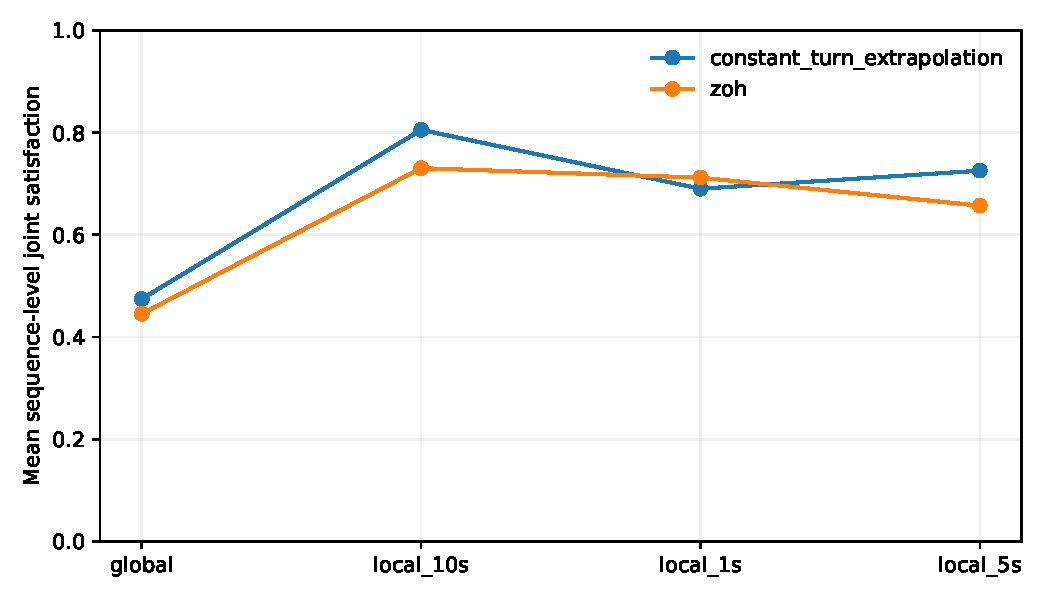
\includegraphics[width=.85\linewidth]{../figures/receiver_robustness.pdf}
\caption{Phase-zero zero-order hold versus causal constant-turn extrapolation. Exact rate/delay/phase rows are in \texttt{receiver\_phase\_per\_sequence.csv}.}
\end{figure}

\section{Causal Receiver Reconstruction}
The alternate receiver starts from the last delivered virtual pose and uses only its delivered corrected speed, yaw rate, source time, and elapsed age to propagate a constant-turn arc. It never accesses future virtual or physical samples. Freshness uses the original source timestamp: extrapolation does not create a new observation. At 2 Hz/200 ms, sequence-mean joint satisfaction changes from zero-order hold to extrapolation by service: global 0.418 to 0.468; local 10 s 0.677 to 0.768; local 5 s 0.599 to 0.672; local 1 s 0.514 to 0.497. Thus receiver choice is not uniformly beneficial. Phase-zero case accounting changes from 31 remediable / six persistent / three already qualified under hold to 26 / six / eight under extrapolation. The main paper retains hold as its primary protocol.

\section{Frozen Configuration Sensitivity}
The deterministic fixed-physics trajectory has one saved run per sequence and is compared against V2 on the same sequences and service contracts. Fixed physics yields 23 remediable, 16 persistent, and one already-qualified case; V2 yields 31, six, and three. All ten fixed-physics global cases remain persistent under ideal available delivery versus six V2 cases. These are paired configuration contrasts, not twenty independent physical sequences. Across 40 cases, mean ideal position discrepancy is 1.289 m for fixed physics versus 0.575 m for V2; mean degraded held-minus-ideal position increments are 0.113 m and 0.186 m, respectively. This diagnostic increment is not an additive causal attribution.

\section{Other Diagnostics and Evidence Boundaries}
A shared score cutoff of 0.80 is diagnostic only because comparator scores have different semantics. The qualification surface is not made monotone: 24/640 adjacent-delay and 44/600 adjacent-rate joint-satisfaction comparisons violate monotonicity, all in the global service. The parking00/parking02 local-versus-global rank reversal is an existence example based on two physical sequences, not a population prevalence estimate. The geofence replay is a null result: sparse occupancy and boundary crossings do not support improved prospective task protection. TerraSentia supports contract feasibility but not zero-shot V2 model superiority. MAGNET supports target-aligned thermal forecast-fidelity characterization only; unverified forecast issuance and availability times prohibit causal delivery, freshness, and remediability conclusions.

\section{Reproduction and Build}
From the repository root, using the Python environment with the analysis dependencies:
\begin{verbatim}
python -m DigitalTwin.analysis.service_timing_budget_study
python -m DigitalTwin.analysis.timing_reviewer_checks
python -m DigitalTwin.analysis.service_timing_robustness
python -m DigitalTwin.analysis.final_timing_paper_figures
python -m pytest tests/test_service_timing_robustness.py -q -p no:cacheprovider
\end{verbatim}
The analysis commands reproduce existing-data outputs; they do not retrain a twin. Once a LaTeX engine is available, compile \texttt{manuscript/main.tex} and this supplement separately from their respective directories with two \texttt{pdflatex} passes each.

\end{document}
